\documentclass[sigplan, review]{acmart}

\usepackage{booktabs} % For formal tables
\usepackage{cleveref}
\usepackage{natbib}


% Copyright
%\setcopyright{none}
%\setcopyright{acmcopyright}
%\setcopyright{acmlicensed}
\setcopyright{rightsretained}
%\setcopyright{usgov}
%\setcopyright{usgovmixed}
%\setcopyright{cagov}
%\setcopyright{cagovmixed}


% DOI
% \acmDOI{10.475/123_4}

% ISBN
% \acmISBN{123-4567-24-567/08/06}

%Conference
\acmConference[PriSC]{Workshop on Principles of Secure Compilation}{January 2018}{Los Angeles, California USA} 
\acmYear{2018}
\copyrightyear{2018}

% \acmPrice{15.00}

%\acmBadgeL[http://ctuning.org/ae/ppopp2016.html]{ae-logo}
%\acmBadgeR[http://ctuning.org/ae/ppopp2016.html]{ae-logo}


\begin{document}
\title{Enforcing Well-bracketed Control Flow and Stack Encapsulation using Linear Capabilities}
% \titlenote{Produces the permission block, and
%   copyright information}
\subtitle{Extended Abstract}
% \subtitlenote{The full version of the author's guide is available as
%   \texttt{acmart.pdf} document}

\author{Lau Skorstengaard}
% \orcid{}
\affiliation{%
  \institution{Aarhus University}
}
\email{lau@cs.au.dk}

\author{Dominique Devriese}
\orcid{0000-0002-3862-6856}
\affiliation{%
  \institution{imec-DistriNet, KU Leuven}
}
\email{dominique.devriese@cs.kuleuven.be}

\author{Lars Birkedal}
\affiliation{%
  \institution{Aarhus University}
}
\email{birkedal@cs.au.dk}

% The default list of authors is too long for headers}
% \renewcommand{\shortauthors}{B. Trovato et al.}


% \begin{abstract}
% This paper provides a sample of a \LaTeX\ document which conforms,
% somewhat loosely, to the formatting guidelines for
% ACM SIG Proceedings. 
% \end{abstract}

%
% The code below should be generated by the tool at
% http://dl.acm.org/ccs.cfm
% Please copy and paste the code instead of the example below. 
%
% \begin{CCSXML}
% <ccs2012>
%  <concept>
%   <concept_id>10010520.10010553.10010562</concept_id>
%   <concept_desc>Computer systems organization~Embedded systems</concept_desc>
%   <concept_significance>500</concept_significance>
%  </concept>
%  <concept>
%   <concept_id>10010520.10010575.10010755</concept_id>
%   <concept_desc>Computer systems organization~Redundancy</concept_desc>
%   <concept_significance>300</concept_significance>
%  </concept>
%  <concept>
%   <concept_id>10010520.10010553.10010554</concept_id>
%   <concept_desc>Computer systems organization~Robotics</concept_desc>
%   <concept_significance>100</concept_significance>
%  </concept>
%  <concept>
%   <concept_id>10003033.10003083.10003095</concept_id>
%   <concept_desc>Networks~Network reliability</concept_desc>
%   <concept_significance>100</concept_significance>
%  </concept>
% </ccs2012>  
% \end{CCSXML}

% \ccsdesc[500]{Computer systems organization~Embedded systems}
% \ccsdesc[300]{Computer systems organization~Redundancy}
% \ccsdesc{Computer systems organization~Robotics}
% \ccsdesc[100]{Networks~Network reliability}


% \keywords{ACM proceedings, \LaTeX, text tagging}

% \begin{teaserfigure}
%   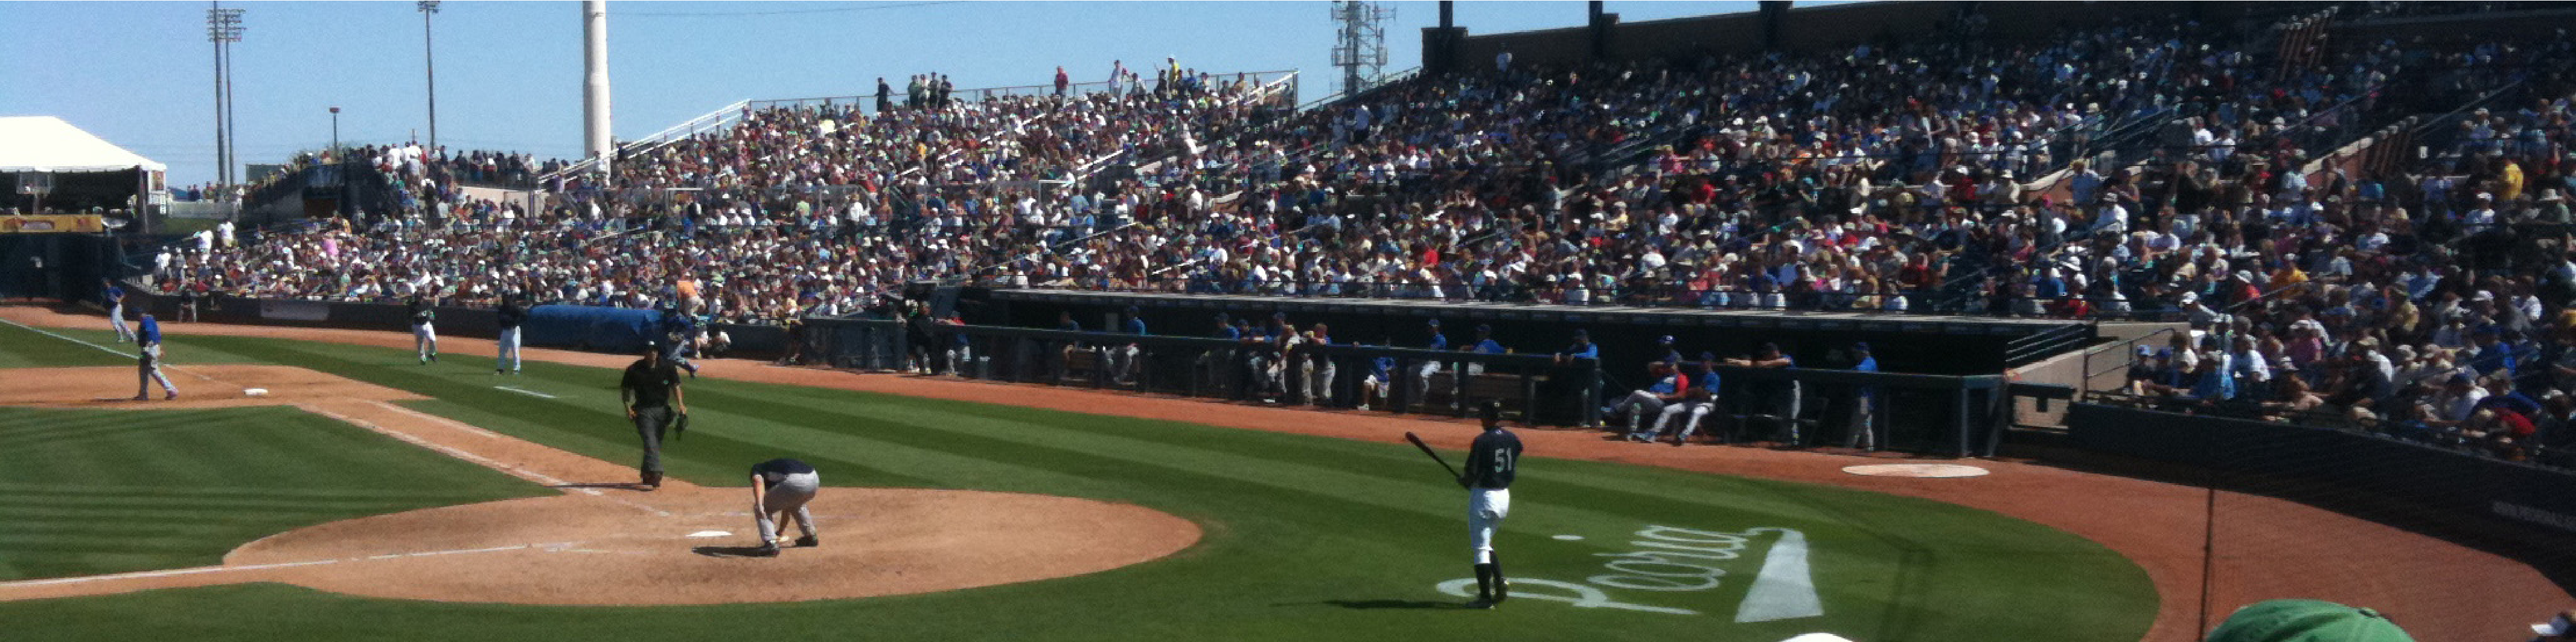
\includegraphics[width=\textwidth]{sampleteaser}
%   \caption{This is a teaser}
%   \label{fig:teaser}
% \end{teaserfigure}


\maketitle

\section{Introduction}
Secure compilers preserve source-language (security-relevant) properties even when the  compiled code interacts with arbitrary target-language components.
Generally, properties that hold in the source language but not in the target language, need to be somehow enforced by the compiler.
Two properties that hold in many high-level source languages, but not in the assembly languages that they are compiled to are the well-bracketedness of control flow and the encapsulation of local state.

Well-bracketed control flow expresses that invoked functions must either return to their callers, invoke other functions themselves or diverge, and generally holds in programming languages that do not offer a primitive form of continuations. 
At the assembly level, this is not so obvious, as invoked functions get direct access to return pointers, that they are supposed to jump to a single time, at the end of their execution, but there is no guarantee that untrusted assembly code respects this intended usage.
Particularly, it may invoke return pointers from other stack frames than the one it was invoked from, either ones from frames higher in the call stack or from stack frames that no longer exist because they have already been returned to before. 

Local state encapsulation is the guarantee that when a function invokes another function, its local variables will not have been modified when the invoked function returns.
At the assembly level, this property is also far from obvious, local variables are stored on the stack when another function is invoked, and functions are not supposed to touch stack frames other than their own.
However, untrusted assembly code is usually not prevented from ignoring this requirement and overwriting the local state of its caller or other stack frames.

To enforce these properties, a target language is needed with some form of security primitive that can be used to prevent untrusted code from misbehaving, without imposing too much overhead on well-behaved code.


\section{Conclusion}

\bibliographystyle{ACM-Reference-Format}
\bibliography{references} 

\end{document}
